\chapter{Benchmarking avec TPC-H}
Le benchmarking TPC-H a été mon deuxième axe de travail avec Oracle, et c'est le sujet de ce chapitre où je présenterai ce qu'est le benchmarking TPC-H, pourquoi nous avons fait cela, et quelle a été ma contribution à cet effort.

\section{Que-est-ce que TPC-H benchmark}

TPC [b.5] est l'acronyme de Transaction Processing Performance Council qui se décrit comme "une organisation à but non lucratif fondée en 1988 pour définir des critères de référence pour le traitement des transactions et les bases de données et pour diffuser des données objectives et vérifiables sur les performances de TPC à l'industrie". Parmi ses membres figurent plusieurs des plus grands fabricants de bases de données.\\
Les benchmarks fournis par cette organisation, qui tentent de simuler autant que possible des situations réelles, ont conduit à une concurrence accrue entre les vendeurs, à la création de bases de données plus rapides et ont incité les fabricants à pousser la technologie jusqu'à ses limites, puisque de bons résultats dans ce domaine constituent un bon argument de vente.\\
TPC-H est l'un des nombreux benchmarks que cette organisation fournit, il est destiné aux systèmes d'aide à la décision. Il consiste en une suite de requêtes Adhoc orientées métier et de modifications concurrentes des données. Les requêtes et les données qui alimentent la base de données ont été choisies de manière à présenter une grande pertinence pour l'ensemble de l'industrie. Ce benchmark illustre les systèmes d'aide à la décision qui examinent de grands volumes de données, exécutent des requêtes avec un degré élevé de complexité et donnent des réponses à des questions commerciales critiques.\\

\textbf{Schéma TPC-H :}
\begin{figure}[H]  
  \centering
    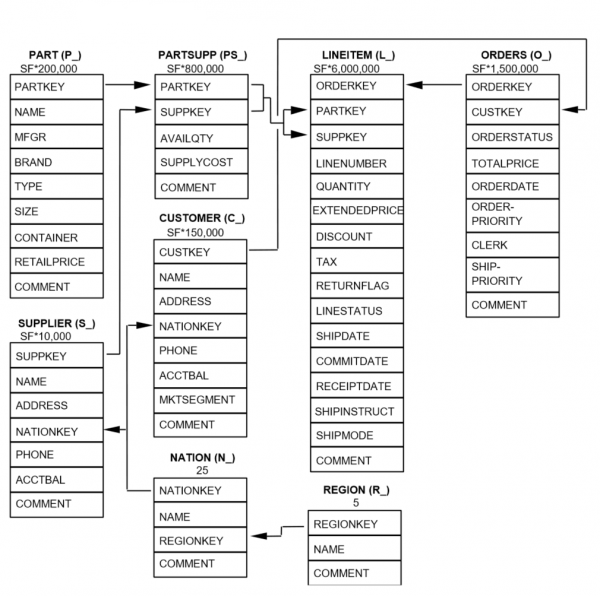
\includegraphics[width=1\textwidth]{chapitre5/Figures/shema_tpch.png}
  \caption{Shéma TPC-H}
\end{figure}

\textbf{Schéma en graph correspondant au schéma TPC-H :}
\begin{figure}[H]  
  \centering
    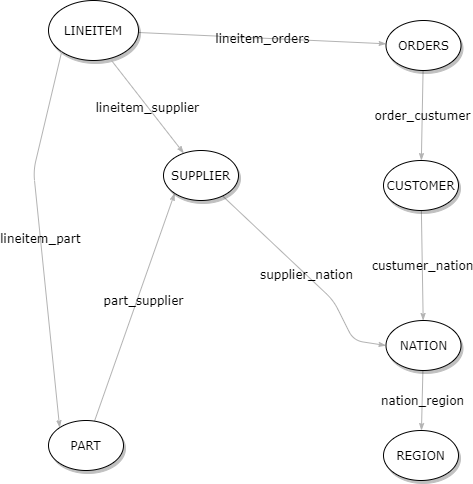
\includegraphics[width=1\textwidth]{chapitre5/Figures/shema_graph.png}
  \caption{Shéma en graphe TPC-H}
\end{figure}

\section{TPC-H dans PGX-D}

Comme presque toutes les requêtes SQL peuvent être associées à une requête PGQL, et que PGX supporte PGQL, il y a beaucoup de potentiel que PGX.D peut apporter au monde OLAP. Grâce à ses hautes performances en mémoire et à son exécution distribuée, il a le potentiel de devenir non seulement un outil d'analyse de graphes pour lequel PGX.D est optimisé, mais aussi un outil d'analyse de bases de données relationnel.

\newpage
\section{Mon travail}
L'exécution des benchmarks TPC-H se fait en plusieurs étapes :

\begin{table}[H]
\centering
\begin{tabularx}{17cm}{|X|X|X|X|}
\hline
\rowcolor[HTML]{3166FF} 
{\color[HTML]{FFFFFF} Generate} & {\color[HTML]{FFFFFF} Transform} & {\color[HTML]{FFFFFF} Load in PGX.D} & {\color[HTML]{FFFFFF} Report} \\ \hline
L'organisation TPC fournit un outil permettant de générer des données avec les facteurs d'échelle souhaités, dans un format qui peut être facilement chargé par des base de données. & Utiliser les données générées pour créer le property graphe correspondant chargéable par PGX. & Charger le graphe dans à chaque fois dans un nombre différent de machines (4, 8, 16) et exécuter les requêtes. & Communiquer les statistiques d'exécution des requêtes, l'utilisation de la mémoire ...etc. \\ \hline
\end{tabularx}
\end{table}

Comme les deux premières étaient déjà faites par un collègue, mon travail s'est concentré sur les deux dernières étapes "Load in PGX.D" et "Report".

\section{Chargement et exécution de requêtes dans PGX.D}
\begin{enumerate}[label=\arabic*)]
\item Cette tâche consistait à exécuter des requêtes TPC-H, des requêtes TPC-H modifiées et des requêtes à domicile avec différents facteurs d'échelle et dans différents nombres de machines pour vérifier la scalabilité de PGX-D avec ce type de charge de travail. Les requêtes TPC-H peuvent être générées à l'aide d'un outil fourni par l'organisation, ces requêtes sont de type SQL, mais les requêtes PGQL, j'ai dû en écrire certaines manuellement et vérifier leur exactitude en les comparant aux résultats de la base de données.
\item Une fois que nous prenons des statistiques sur la consommation mémoire d'un graphe donné dans le système PGX, le chargement de toutes les propriétés devient inutile. C'est pourquoi j'ai créé un script python pour générer automatiquement des fichiers de configuration, afin de pouvoir charger uniquement les propriétés nécessaires à l'exécution de la requête, ce qui a augmenté mon efficacité puisque le chargement du graphe avec moins de propriétés prend moins de temps. Par exemple charger un graphe de l’échelle SF100 avec toutes les propriétés inclues demandait a peu prés 40 minutes stricte avec huit machines de plus de 24 cœurs chacune, car plus de 100Go devait être chargé en mémoire, avec ma solution, cela pourrait prendre de 20 à 40 min.
\item Enfin, j'ai fait évoluer les benchmarks de l'exécution des requêtes à l'aide du shell Groovy (un shell client supporté par PGX aux côtés de jShell et d'un shell python) vers l'utilisation de jShell puisque l'équipe PGX a abandonné le support pour le premier.
\end{enumerate}

\section{Reporting}
La tâche de reporting consistait principalement à analyser le fichier journal du serveur pour extraire automatiquement les statistiques souhaitées lorsque l'exécution de toutes les requêtes se termine et à les afficher pour que les membres de l'équipe plus spécialisés puissent les analyser.\\

\begin{figure}[H]  
  \centering
    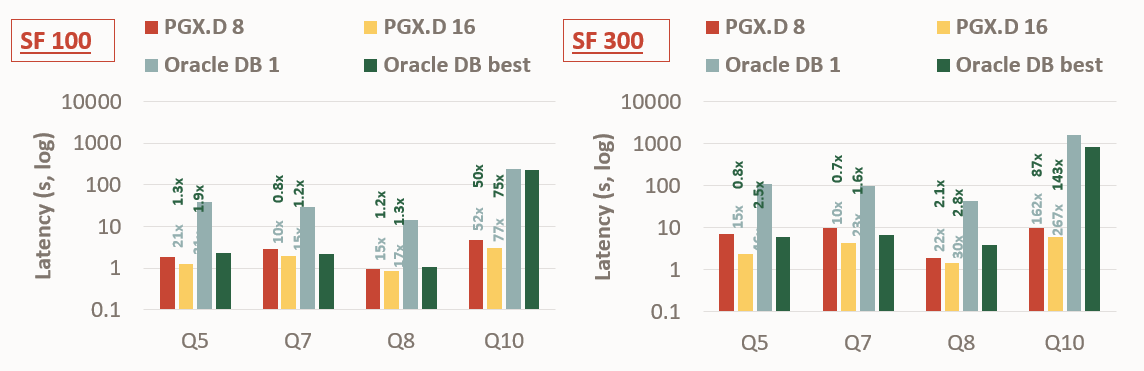
\includegraphics[width=1.15\textwidth]{chapitre5/Figures/TPC-H.PNG}
  \caption{Benchmark TPC-H, comapraison entre Oracle DB et PGX.D avec des requêtes lourds en jointures, avec les charges SF 100 et SF 300}
\end{figure}

La figure 5.3 montre une partie des résultats que j’ai reporté. Ces résultats montrent que TPC-H offre un temps d’exécution largement plus faible que celui d’Oracle dans ces meilleurs cas quand les requêtes sont lourds en jointures et que la charge et plus grande car en peut voir que la différence augmente avec SF 300 par rapport à la charge moins lourd SF 100.\\
Cette grande différence et due au fait que PGX.D par sa structure des graphes gère mieux les charges avec beaucoup des jointures et génère moins des résultats intermédiaires par rapport ou requêtes SQL en Oracle DB, quand ces résultats intermédiaires ne peuvent pas tenir en mémoire, le système d’exploitation commence à vider la mémoire RAM dans le disque qui est une tâche assez lourde pour le CPU.